\documentclass{article}
\usepackage[utf8]{inputenc}
\usepackage[margin = 0.8in]{geometry}
\usepackage{graphicx}
\usepackage{amsmath, amssymb}
\usepackage{subcaption}
\usepackage{multirow}
\usepackage{mathtools}
\usepackage{float}


\title{RBE549 - Homework 5}
\author{Keith Chester}
\date{Due date: October 6, 2022}

\begin{document}
\maketitle

\section*{Problem 1}

In this problem we are looking at how the SURF algorithm integral images quickly. To this end we will be demonstrating how to compute the sum of a rectangular regon of an image using only a $3$ operations - $+ and -$. An example image of the region is:

\begin{figure}[H]
    \centering
    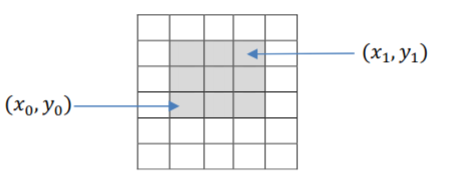
\includegraphics[width = 0.45\textwidth]{imgs/prob1.png}
    \caption{Edges and verticies}
    \label{fig:prob1-1}
\end{figure}

Based on the method and direction that the integral image was calculated, we can identify key squares that we can utilize to do our calculation - $P$, $Q$, $S$, and $R$:

\begin{figure}[H]
    \centering
    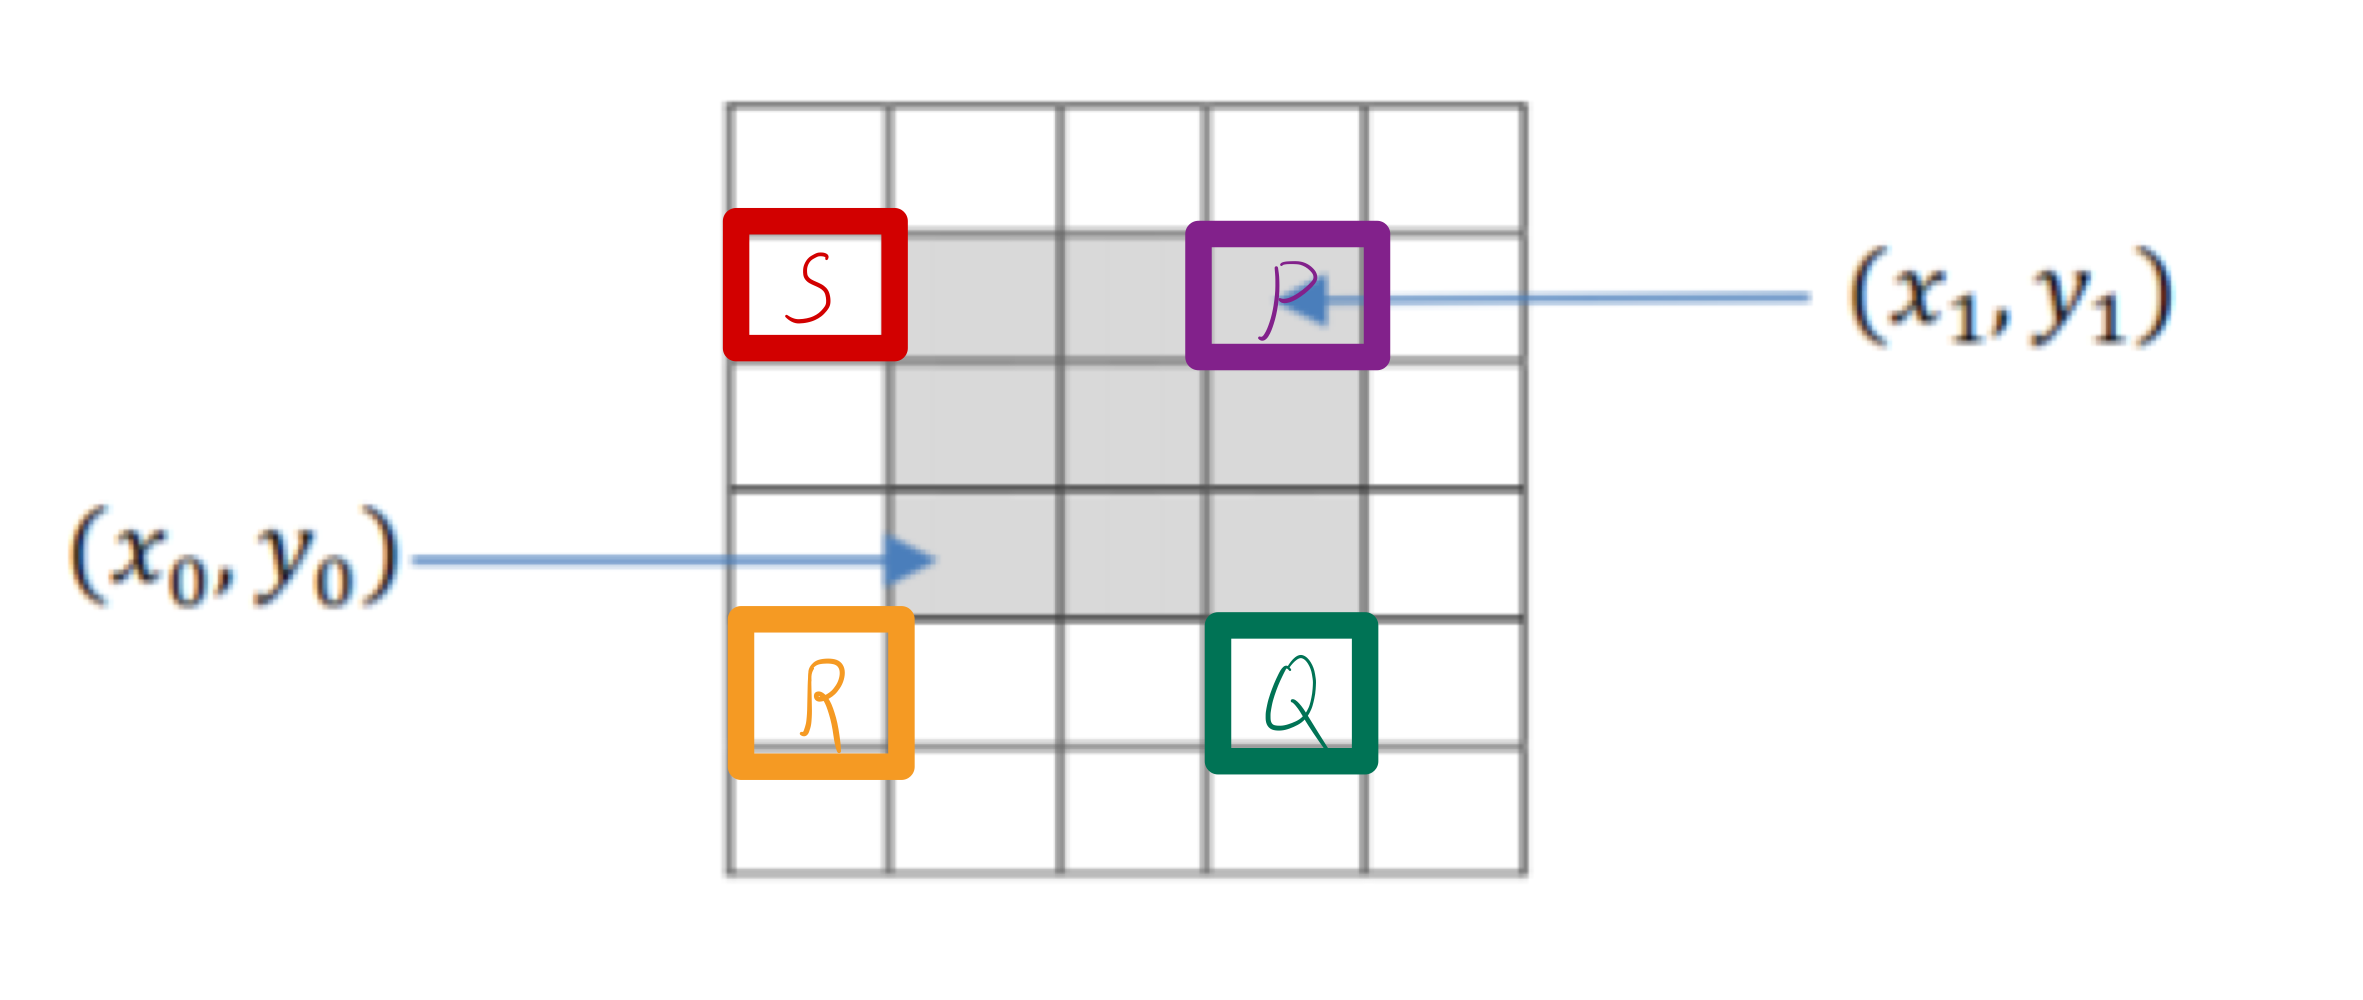
\includegraphics[width = 0.45\textwidth]{imgs/psqr.png}
    \caption{P, Q, S, and R identification}
    \label{fig:prob1-2}
\end{figure}

From here we can identify each of $P$, $Q$, $S$, and $R$ via their positions relative to our initial definitions of our region, $(x_0, y_0)$ and $(x_1, y_1)$:

\begin{itemize}
    \item $P=(x_1, y_1)$
    \item $Q=(x_1, y_0 - 1)$
    \item $S=(x_0-1, y_1)$
    \item $R=(x_0-1, y_1-1)$
\end{itemize}

With these values you can calculate the sum of the given region by performing the following calculation:

\begin{equation}
    I_\Sigma[i,j] = P - Q - S + R
\end{equation}

\section*{Problem 2}

In this section we are tackling problems with quad trees.

\subsection*{A}

We are tasked with creating an image from the quad tree output of $[[0110]10[0100]]$. The image would be presented below:

\begin{center}
    \begin{tabular}{ | c | c | c | c | }
        \hline
        0 & 1 & 1 & 1 \\ 
        \hline
        0 & 1 & 1 & 1 \\ 
        \hline
        0 & 1 & 0 & 0 \\ 
        \hline
        0 & 0 & 0 & 0 \\ 
        \hline  
    \end{tabular}
\end{center}

\subsection*{B}

Now we're tasked with shifting the image left, with the rightmost column containing all zeroes, and then determining the resultant quad tree encoding. The expected image would be:

\begin{center}
    \begin{tabular}{ | c | c | c | c | }
        \hline
        1 & 1 & 1 & 0 \\ 
        \hline
        1 & 1 & 1 & 0 \\ 
        \hline
        1 & 0 & 0 & 0 \\ 
        \hline
        0 & 0 & 0 & 0 \\ 
        \hline  
    \end{tabular}
\end{center}

\noindent ...this would encode to $[1[1001]0[1000]]$.

\subsection*{C}

In this problem, we are asked to describe a recursive algorithm to rotate a quad tree. For instance, given our original quad tree from section A:

\begin{center}
    \begin{tabular}{ | c | c | c | c | }
        \hline
        0 & 1 & 1 & 1 \\ 
        \hline
        0 & 1 & 1 & 1 \\ 
        \hline
        0 & 1 & 0 & 0 \\ 
        \hline
        0 & 0 & 0 & 0 \\ 
        \hline  
    \end{tabular}
\end{center}

\noindent This had a quad tree encoding of $[[0110]10[0100]]$. If we were to rotate this image $90^\circ$ clockwise:

\begin{center}
    \begin{tabular}{ | c | c | c | c | }
        \hline
        0 & 0 & 0 & 0 \\ 
        \hline
        0 & 1 & 1 & 1 \\
        \hline
        0 & 0 & 1 & 1 \\
        \hline
        0 & 0 & 1 & 1 \\
        \hline
    \end{tabular}
\end{center}

\noindent This has a quad tree encoding of $[[0010][0011]10]$. Code for this recursive approach can be found in $problem2.py$.

A description of it loosely: For each node of the quad tree, change the order of the tree to be last, then first through third. Add these nodes to the new resulting tree, but call the same rotation function on each child. If a node is a singular number (meaning all values within the quad tree are the same from that point on) you can just return that value back.

\section*{Problem 3}

In this problem we aim to prove that rotating and translation an entire point cloud does not affect the distance between any two of the points within, or that $||\vec{x}^0_1-\vec{x}^0_0|| = ||\vec{x}^1_1 - \vec{x}^1_0||$. We will let $\vec{x}^1_i=R\vec{x}^0_i + \vec{T}$.

First, we state our initial equation with the above definitions:

\begin{equation}
    ||\vec{x}^1_1 - \vec{x}^1_0|| = ||(R\vec{x}^0_1+\vec{T}) - (R\vec{x}^0_0 + \vec{T})||
\end{equation}

\noindent ...this we can expand and simplify and then get rid of the effect of our translation $\vec{T}$:

\begin{equation}
    ||\vec{x}^1_1 - \vec{x}^1_0|| = ||R\vec{x}^0_1+\vec{T} - R\vec{x}^0_0 - \vec{T}||
\end{equation}

\begin{equation}
    ||\vec{x}^1_1 - \vec{x}^1_0|| = ||R\vec{x}^0_1 - R\vec{x}^0_0||
\end{equation}

\noindent This is equivlanet to the form:

\begin{equation}
    ||\vec{x}^1_1 - \vec{x}^1_0|| = ||R|| * ||\vec{x}^0_1 - \vec{x}^0_0||
\end{equation}

\noindent $||R|| = R^TR$, and $R^TR = 1$, so therefore:

\begin{equation}
    ||\vec{x}^1_1 - \vec{x}^1_0|| = ||\vec{x}^0_1 - \vec{x}^0_0||
\end{equation}

\noindent This proves that the resulting distance between two moved points would be calculated the same.


\section*{Problem 4}

In this section, we are presented with the following segmented map with class labels:

\begin{center}
    \begin{tabular}{ | c | c | c | c | c | }
        \hline
        1 & 0 & 0 & 0 & 1 \\ 
        \hline
        1 & 1 & 1 & 1 & 1 \\ 
        \hline
        1 & 0 & 1 & 0 & 1 \\ 
        \hline
        1 & 0 & 0 & 0 & 1 \\ 
        \hline
        1 & 2 & 2 & 2 & 1 \\ 
        \hline  
    \end{tabular}
\end{center}

\subsection*{A}

Here we aim to list all regions and their classes, and edges and which regions they separate:

\begin{figure}[H]
    \centering
    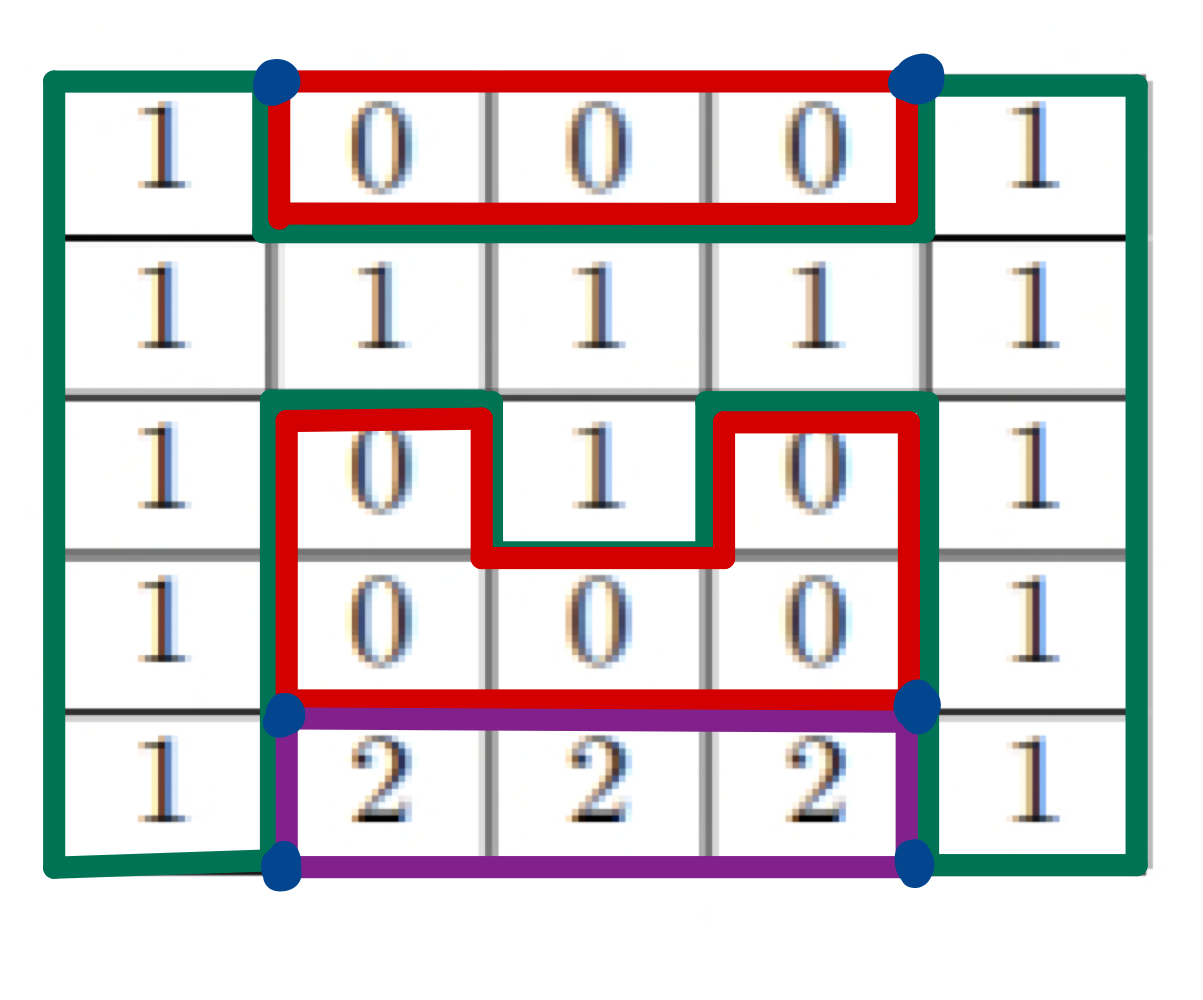
\includegraphics[width = 0.45\textwidth]{imgs/edges_verticies.png}
    \caption{Edges and verticies}
    \label{fig:edges_verticies}
\end{figure}

From this we can find the following regions and edges:

\begin{center}
    \begin{tabular}{ | c | c | }
        Region & Class \\
        \hline
        -1 & -1 \\
        0 & 1 \\
        1 & 0 \\
        6 & 0\\
        9 & 2 \\
    \end{tabular}
\end{center}

\begin{center}
    \begin{tabular}{| c | c | c |}
        Edge & Class & Regions \\
        \hline
        1 & -1 & 1 \\
        2 & -1 & 0 \\
        3 & 0 & 1 \\
        4 & 1 & 2 \\
        5 & 0 & 1 \\
        6 & 0 & 2 \\
        7 & 1 & 2 \\
        8 & -1 & 2 \\
        9 & -1 & 1
    \end{tabular}
\end{center}

\subsection*{B}

We are asked here how many verticies are in this diagram. As labeled in the figure above, there are six verticies.

\subsection*{C}

We are then asked if this is eight- or four- connected. This work could be either; there are no diagonals that would demonstrate an eight-connected setup, but that doesn't exclude it since eight-connected is a subset of four-connected.


\end{document}